% !TeX root = ../main.tex

\subsection*{ISOMAP Algorithm}
A non-linearity ``patch'' to MDS

\begin{figure}[H]
	\centering
	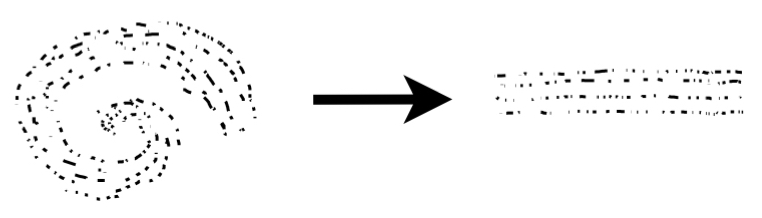
\includegraphics[width=0.5\textwidth]{isomap}
\end{figure}

\paragraph{Idea:} Nearby points have their ``usual'' euclidian distance. If a pair of points are not within a local neigbourhood, then the distance between these points is a \textbf{graph distance}\footnote{Compute the all pairs shortest path (Dejkstra, A*,  DFS, Floyd–Warshall, ...)}. Then run MDS on the resulting distance Matrix.

ISOMAP operates on geodesic distances (like a distance on earths surface/distances on the manifold).

\subsubsection*{Additional notes}
\begin{itemize}
    \item Manifold learning algorithms are based on the idea that the dimensionality of many data sets is only artificially high. Although the data points may consist of thousands of features, they may be described as a function of only a few underlying parameters. That is, the data points are actually sampled from a low-dimensional manifold that is embedded in a high dimensional space. Manifold learning algorithms attempt to uncover these parameters in order to find a low-dimensional representation of the data.
    \item Error function: \[E = ||\text{inner product distances in graph} - \text{inner product distances in new coordinate system}||_{L_2}\]
    \item Finding optimal dimensionality: Look at residual variance (or error) (depending on \(d\)) and search for "elbow" at which the curve ceases to decrease significanlty with added dimensions. (PCA/MDS tend to overestimate dimensionality)
    \item PCA and MDS are guaranteed, given sufficient data, to recover the true structure of linear manifolds
    \item ISOMAP is guaranteed asymptotically to recover the true dimensionality and geometric structure of a strictly larger class of nonlinear manifolds, which intrinsic geometry is that of a convex region of Euclidean space
    \item ISOMAP is a polynomial time, noniterative procedure which guarantees global optimality
    \item Possible problems:

        \begin{itemize}
            \item If \(k\) for \(k\)-NN is to large, or noise in the data moves the points slightly off the manifold, ISOMAP is vulnerable to "short-circuiut error", where even single errors can alter the low-dim embedding drastically
            \item If \(k\) is to small, the neighborhood graph may become too sparse to approximate geodesic paths accuratly
        \end{itemize}

\end{itemize}
